\documentclass[a4paper,12pt]{article}

\usepackage[czech]{babel}
\usepackage[utf8]{inputenc}
\usepackage{indentfirst}
\usepackage{hyperref}
\usepackage{graphicx}

\newcommand{\priloha}[1]{\section*{#1}\addcontentsline{toc}{section}{#1}}

\title{Uživatelská dokumentace programu Damebot}
\author{Václav Stupka}
\date{2. února 2022}

\begin{document}
	\maketitle
	\tableofcontents
	
	\section{Úvod}
	Damebot je program, díky kterému si můžete zahrát dámu proti počítači. Tento projekt vznikl jako zápočtový program
	pro předmět Programování pro pokročilé v~zimním semestru prvního ročníku na Matematicko-fyzikální fakultě Univerzity
	Karlovy (obor Informatika). Neočekávejte proto nijak převratně chytrý herní algoritmus ani propracovanou moderní grafiku.
	Přesto se domnívám, že pro méně zkušené hráče dámy bude tento program zdrojem zábavy a možná také menší výzvou.
	
	Tento dokument slouží především jako uživatelská dokumentace. Naleznete zde postup instalace programu, způsob spuštění,
	ovládání a pro připomenutí také pravidla dámy (ačkoli jsem se snažil respektovat pravidla české dámy, je možné, že se
	mi to ne vždy podařilo).
	
	\section{Instalace a spuštění}
	Program Damebot je možné stáhnout na adrese
	\url{https://github.com/basvas-jkj/dame_bot/blob/main/download/dame_bot.zip}.
	Zde stačí kliknout na tlačítko \textit{download} (nebo odkaz \textit{View raw}). Stažený soubor \textit{damebot.zip} otevřete
	a extrahujte jeho obsah. Tím je instalace dokončena.
	
	Pro spuštění programu otevřete rozbalenou složku \textit{damebot} a klikněte na soubor \textit{index.html}
	(nebo \textit{index}). Damebot se otevře ve webovém prohlížeči, který máte nastavený jako výchozí.
	
	\section{Ovládání}
	V~programu Damebot vždy hrajete bílými kameny. Klikněte na ten kámen, kterým chcete táhnout. Pole pod tímto kamenem
	zčervená. Následně klikněte na prázdné pole, na které chcete označený kámen přemístit. Pokud je tento tah podle
	pravidel hry možný, kámen se přemístí na zvolené pole a odznačí se. Dále je na tahu protivník (tedy Damebot). Který
	hráč je zrovna na tahu, můžete sledovat nad šachovnicí.
	
	V~případě, že jste označili některý ze svých kamenů, ale následně jste klikli na pole, na které tento kámen táhnout
	nemůže, nic se nestane. Můžete zvolit jiné pole. Pokud kliknete na jiný ze svých kamenů, označíte ho. Původní kámen se odznačí. Označený kámen se odznačí také v~případě, že kliknete na bílé pole nebo když myší opustíte plochu šachovnice.
	V~případě vícenásobného skoku je kámen označený až do chvíle, kdy je vícenásobný skok dokončen.
	
	Provedené tahy není možné žádným způsobem vrátit. Výjimkou je pouze vícenásobný přeskok: pokud kliknete na bílé pole,
	jiný vlastní kámen nebo pokud opustíte myší šachovnici, skákající kámen se vrátí do původní pozice. Pokud je však
	vícenásobný skok dokončen, nelze ho již vrátit zpět (totéž platí i pro ostatní tahy).
	
	Damebot neprovede svůj tah okamžitě. Nejprve chvíli počká, poté označí modře pole, na kterém stojí kámen, kterým hodlá
	táhnout. Modře se označí také pole, na které příslušný kámen chystá přemístit (v~případě vícenásobného skoku se
	zvýrazní všechna pole, přes která kámen přejde). Následně se všechna zvýrazněná pole odznačí a příslušný kámen
	se sám přesune. Díky tomu máte možnost lépe sledovat, který kámen se přesunul a na které pole.
	
	V~případě výhry jednoho z~hráčů se nad šachovnicí objeví nápis \textit{White wins}, resp. \textit{Black wins}. Remízu
	program žádným způsobem nesleduje (není omezený ani počet tahů -- partie může být teoreticky nekonečná). Pokud si
	budete chtít zahrát novou partii, kliněte na tlačítko \textit{New game}. To můžete udělat na konci hry i v~jejím
	průběhu.
	
	\section{Pro pokročilé}
	Pokročilí uživatelé mohou mít zájem se podívat také na zdrojový kód programu, případně si vytvořit vlastní modifikaci.
	Patříte-li mezi ně, navštivte webovou stránku projektu \url{https://github.com/basvas-jkj/dame_bot}, kde ve složce
	\textit{docs} naleznete programátorskou dokumentaci s~dalšími potřebnými informacemi.
	
	\priloha{Příloha 1 -- pravidla dámy}
	Dáma se hraje na šachovnici (velikost 8×8 polí) se sadou 12~bílých a 12~černých kamenů. Kameny jsou na začátku hry
	rozmístěny v~prvních třech řadách na černých polích (o přípravu hry se stará Damebot). Hru začíná bílý. Kameny se
	pohybují o jedno pole úhlopříčně směrem vpřed (v~tomto případě bílé kameny nahoru a černé dolů). Jestliže je toto
	pole obsazené protivníkovým kamenem a další pole ve stejném směru je volné, může na toto pole posunout svůj kámen.
	Přeskočený kámen je tímto vyhozen a odebrán ze šachovnice. Takový skok je možné provést vícekrát (lze tedy vyhodit
	několik soupeřových kamenů najednou), vždy však musí skákat tentýž kámen (v~jednom tahu nelze provést více skoků
	různými kameny).
	
	Pokud má hráč možnost vyhodit libovolný soupeřův~kámen, je povinen tak učinit. Má-li možnost skákat více kameny,
	může si vybrat kterýkoli z~nich (právě jeden). Rovněž si hráč může vybrat, které kameny přeskočí. Jestliže se hráč
	rozhodne pro vícenásobný skok, musí jej hráč provést celý (skok tedy musí skončit pozicí, ve které skákající kámen
	nemůže vyhodit žádný další protivníkův~kámen).
	
	Kámen, který se dostane na opačný okraj šachovnice, se promění v~dámu. Dáma se může pohybovat úhlopříčně všemi čtyřmi
	směry o libovolný počet polí. Skákat může dáma i přes kameny, které s~ní přímo nesousedí, a skok může ukončit na
	libovolném poli za přeskočeným kamenem (na stejné diagonále). Pokud z~tohoto pole může dále skákat, je povinna tak
	učinit. Při tom může změnit směr. Přes jeden kámen opačné barvy nesmí dáma skočit vícekrát. Toto se nevztahuje na prázdná
	pole (je tedy možné např. začít a skončit tah na stejném poli).
	
	Přes kámen stejné barvy není povoleno skákat (platí pro obyčejné kameny i pro dámu). Pokud se běžný kámen dostane
	na poslední řadu skokem, promění se v~dámu a tah \textbf{končí} (i v~případě, že by proměněná dáma mohla pokračovat
	ve skoku).
	
	Hra končí ve chvíli, kdy jeden z~hráčů přijde o všechny svoje kameny nebo nemůže zahrát další tah (všechny jeho kameny
	jsou zablokované). Vítězem je pak jeho protivník. Remíza by nastala v~případě, kdy při bezchybné hře není ani jeden
	z~hráčů schopen vyhodit nebo zablokovat všechny soupeřovy kameny (např. pokud oběma hráčům zbyde jedna dáma).
	Damebot však tuto možnost nesleduje, hráč se tedy musí sám rozhodnout, zda má smysl v~partii pokračovat.
	
	Na závěr ještě poznamenám, že tato pravidla platí i pro fyzického hráče, i pro Damebota.
	\\
	\\
	\\
	\\
	\\
	\\
	\\
	\\
	\\
	
	\priloha{Příloha 2 -- ukázka programu}
	\begin{figure}[h]
		\centering
		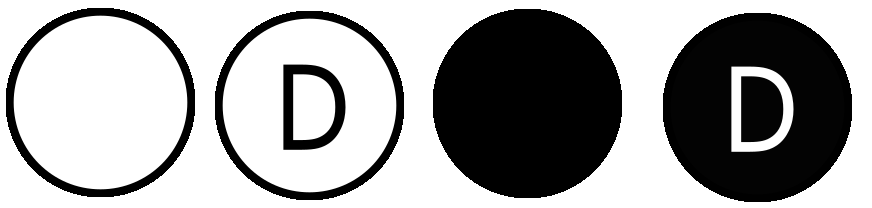
\includegraphics{img/kameny}
		\caption{Zleva bílý kámen, bílá dáma, černý kámen, černá dáma}
	\end{figure}

	\begin{figure}[h]
		\centering
		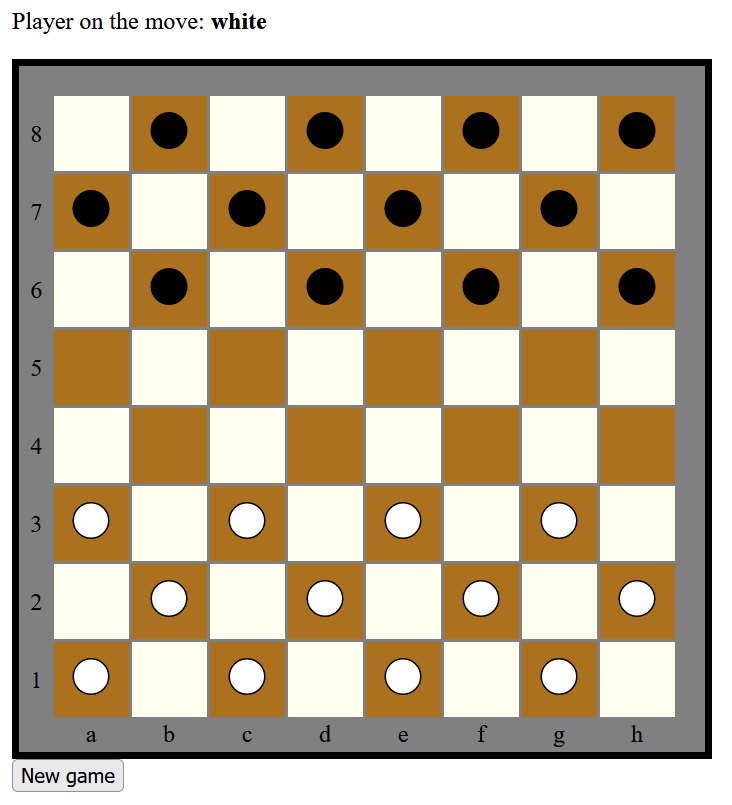
\includegraphics{img/vychozi_pozice}
		\caption{Výchozí pozice}
	\end{figure}

	\begin{figure}[h]
		\centering
		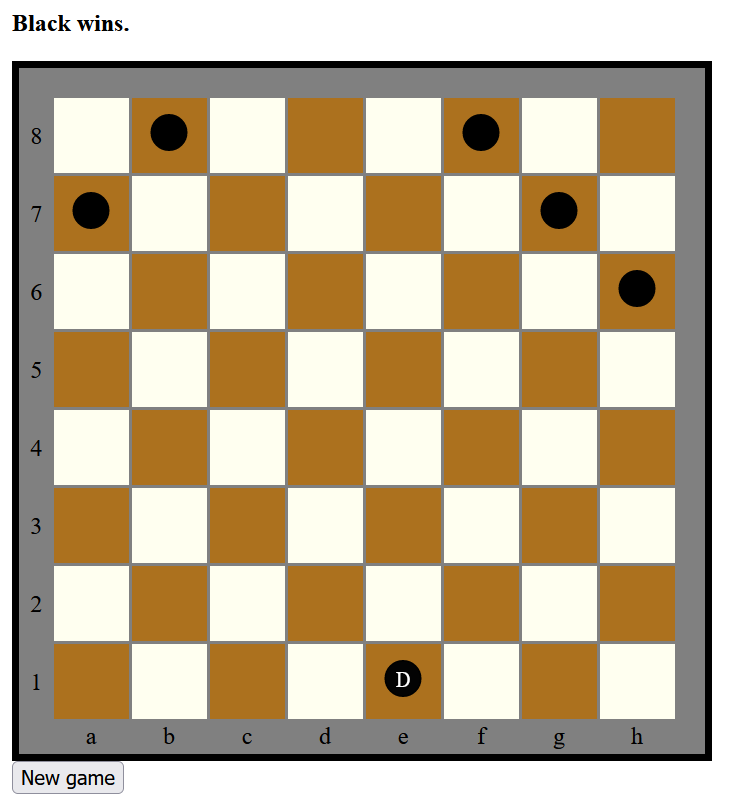
\includegraphics{img/bot_vyhral}
		\caption{Pozice, ve které černý (Damebot) zvítězil.}
	\end{figure}

	\begin{figure}[h]
		\centering
		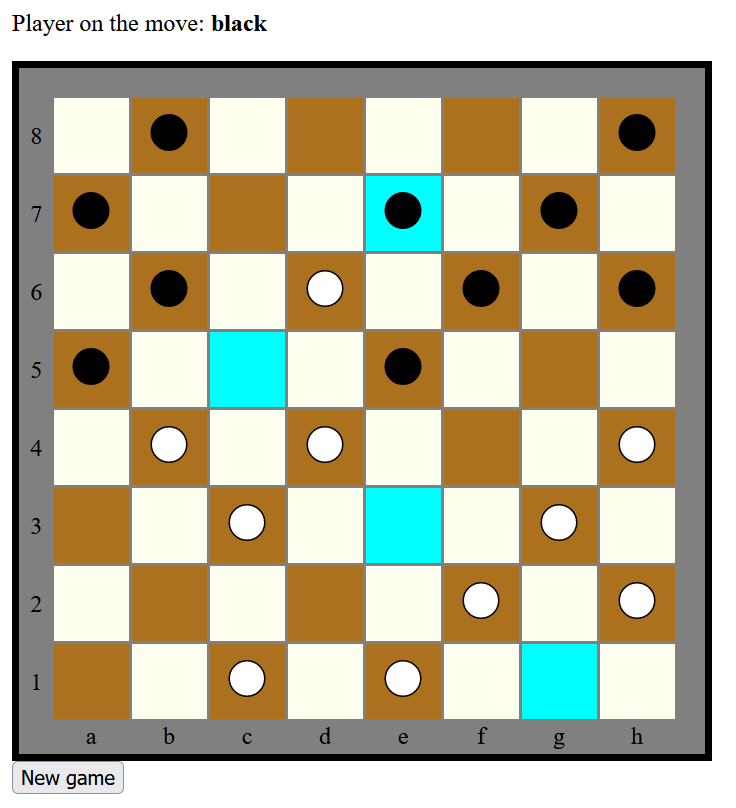
\includegraphics{img/trojnasobny_skok}
		\caption{Damebot se chystá k trojnásobnému skoku.}
	\end{figure}
\end{document}